%
% curso-latex-forma-2020.tex
%
% LaTeX para Linguistas
% ForMA — IEL/Unicamp
% 17, 24 e 31 de julho de 2020
%
%

% História e filosofia
%
% - TeX: invenção de Donald Knuth
% - O projeto começa em 1977, com a segunda edição de The Art of Computer
% Programming e se estende pelos próximos dez anos
% - LaTeX: conjunto de macros por Leslie Lamport

% O LaTeX é uma linguagem de marcação
%
% O LaTeX é uma linguagem de markup, ou marcação de texto. Você deve instruir o computador sobre como o texto deverá ser formatado. Os comandos em LaTeX são semânticos, ou seja, informam que tipo de conteúdo o texto representa. Por exemplo, intuitivamente, o que fazem os comandos a seguir?
%
% \tableofcontents
% \section{Introdução}

% Estrutura deste curso
%
% Este curso está contido (praticamente) em apenas um arquivo e o código começa logo abaixo. A ideia é que este arquivo também sirva de exemplo para a confecção de um artigo. Primeiramente, veremos a estrutura de um arquivo .tex (preâmbulo e corpo do documento) e em cada seção nos atentaremos a % um aspecto do LaTeX.

% Preâmbulo
\documentclass[10pt,a4paper,oneside]{article}
\usepackage{polyglossia}
  \setdefaultlanguage[variant=brazilian]{portuguese}
  \setotherlanguage{english}
\usepackage[dvipsnames]{xcolor}
\usepackage{microtype,xspace,multicol,minted,emoji}
\usepackage{hyperref}
  % Links com cores menos chamativas
  \hypersetup{
    colorlinks = true,
    citecolor  = MidnightBlue,
    linkcolor  = MidnightBlue,
    urlcolor   = MidnightBlue}
\usepackage[breakable]{tcolorbox}
%\usepackage{showframe,fullpage,setspace}
\usepackage{enumitem}
\usepackage{booktabs,longtable}
\usepackage{graphicx}
% \usepackage[alf]{abntex2cite}
\usepackage{tipa,vowel,linguex}
\newfontfamily\ipafont{Doulos SIL}
\usepackage[linguistics]{forest}

% Metadados
\title{\LaTeX{} para linguistas}
\author{Rafael Beraldo\\ \ForMA — IEL/Unicamp}
\date{17, 24 e 31 de julho de 2020}

% Meus comandos
\newcommand\ForMA{\textsf{ForMA}\xspace}
\newmintinline[code]{latex}{autogobble}
\newcommand\eng[1]{\emph{\foreignlanguage{english}{#1}}}

% Ambiente para exemplos
\newtcolorbox[auto counter,number within=section]{examplebox}{
  % width=.8\textwidth,
  fonttitle=\sffamily\small,
  colframe=gray!70!white,
  colback=gray!10!white,
  coltitle=black!80!white,
  box align=center,
  center title}
  % title=Exemplo~\thetcbcounter}
\newenvironment{example}
{\begin{center}\begin{examplebox}}
{\end{examplebox}\end{center}}

% Documento em si
\begin{document}
\frenchspacing

\maketitle

\begin{abstract}
  Curso virtual de \LaTeX{} para linguistas oferecido pelo \ForMA — Núcleo de Estudos em Gramática Formal, Mudança e Aquisição do Instituto de Estudos da Linguagem (IEL), Unicamp — nos dias 17, 24 e 31 de julho de 2020. O curso é uma adaptação para o ambiente virtual da versão presencial, que pode ser \href{https://github.com/rberaldo/workshop-latex-forma}{encontrada no Github}. A intenção é que se leia o código-fonte, pois ele contém comentários explicativos importantes.
\end{abstract}

\tableofcontents

\section{Classes e compilação}
% Objetivos:
% - Diferenças entre classes e implicações
% - Comandos: \documentclass, \section
% - Compilação de um documento
% - Compiladores: pdflatex, lualatex, xelatex
% - Erros de compilação

Arquivos \texttt{.tex} começam com um cabeçalho (também chamado de \emph{preâmbulo}) que contém informações básicas sobre o documento, como tipo (artigo, livro, carta etc.), metadados e carregamento de pacotes que expandem as funções do \LaTeX.

A classe deste arquivo é \texttt{article} e, por isso, conseguimos usar o ambiente \texttt{abstract}. Vamos remover esse ambiente e mudar a classe para \texttt{book} e ver o que acontece com o número das seções. Vamos observar também como compreender erros na compilação, mantendo o ambiente de resumo.

\section{Comandos e espaços em branco}
% Objetivos:
% - Aprender sobre espaço em branco
% - Reconhecer dois tipos de comando: com e sem argumentos

Espaços em branco não são tomados literalmente no \LaTeX:     esses       vários    espaços         serão       condensados      em apenas     um espaço    em branco.

Assim, o uso de espaços no código-fonte separa palavras e comandos e deve seguir melhores práticas que são aprendidas com o tempo, leitura do código de outras pessoas e desenvolvimento de um estilo pessoal.

Certos comandos, como \code+\tableofcontents+ são simples, ou seja, não têm argumentos. Já comandos como \code+\section{Introdução}+ recebem argumentos, assim como verbos têm valência. Para o \LaTeX, não há muita diferença entre…

\begin{example}
  \centering
  \code+\section{Introdução}+ e\\
  \code+\section {Introdução}+
\end{example}

…mas por que a primeira versão é mais adequada do ponto de vista humano?

\subsection{Exercício: espaços em branco}
% Problema: o espaçamento deste texto está catastrófico. Existem espaços sobrando ou faltando, tanto entre as palavras quanto entre os parágrafos. O texto final deve conter quatro parágrafos, sendo o segundo uma lista cujos itens são separados por novas linhas.

Acima de tudo, é fundamental ressaltar que o julgamento imparcial das eventualidades maximiza as possibilidades por conta das direções preferenciais no sentido do progresso. Desta maneira,a complexidade dos estudos efetuados cumpre um papel essencial na formulação das condições financeiras e administrativas                       exigidas, que são três:
1. O mundo atual.
2. Os amigos de família.
3. A importância dos mercados mundiais.
Nunca é demais lembrar o peso e o significado destes problemas, uma vez que o fenômeno da Internet exige a precisão e a definição do processo de comunicação como um todo. No entanto, não podemos esquecer que                    a consulta aos diversos militantes agrega valor ao estabelecimento das regras de conduta normativas.Do mesmo modo, o acompanhamento das preferências de consumo garante a contribuição de um grupo importante na determinação das novas proposições.
O empenho em analisar o desenvolvimento contínuo de distintas formas de atuação aponta para a melhoria do sistema de participação geral.

\section{Símbolos especiais}
% Objetivos:
% - Aprender sobre aspas, hifens, travessões e espaços não quebráveis
% - Entender que certos caracteres não são usados literalmente

\begin{description}
  \item[Aspas] Não usamos as chamadas “aspas burras” (\code+""+):

  \begin{example}
    ``Abrimos aspas com dois acentos graves e fechamos com duas aspas simples.''
  \end{example}

  \item[Hífen, travessão e meia-risca] Existe uma diferença entre o hífen, o travessão e a meia-risca:

  \begin{example}
    Leve um guarda-chuva --- ouvi na rádio que pode chover entre 10h--13h.
  \end{example}

  \item[Espaços não quebráveis] Às vezes, é necessário que um espaço não se quebre ao fim de uma linha, por exemplo:

  \begin{example}
    Às 10~horas de ontem…\\
    Fui à casa do Sr.~Silva…\\
    Veja mais na página~40.
  \end{example}

  \item[Caracteres reservados] Os símbolos a seguir estão reservados:

  \begin{example}
    \verb+# $ % ^ & _ { } ~ \+
  \end{example}

  Devemos escapá-los, ou seja, precedê-los por uma barra \code+\+, para que sejam impressos da maneira correta:

  \begin{example}
    \# \$ \% \^{} \& \_ \{ \} \~{} \textbackslash
  \end{example}
\end{description}

\subsection{Exercício: caracteres reservados}
% Problema: se as linhas a seguir forem descomentadas, o documento não irá compilar corretamente, pois os símbolos reservados ao LaTeX estão sendo usados incorretamente. Descomente as linhas e corrija os problemas até que a compilação seja bem-sucedida.

(Descomente as linhas a seguir:)

% Nossos teclados são bem limitados em termos de símbolos. Provavelmente por isso, os poucos símbolos que temos à nossa disposição foram tomando sentidos diferentes com o passar do tempo.

% É muito comum, por exemplo, substituir a letra~“e” pelo~&. Em alguns contextos na Internet, a~# é usada para indicar etiquetas. Em alguns casos, _underlines_ marcam itálico. E no \LaTeX, o símbolo~\ indica o começo de um comando.

\section{O preâmbulo do documento}
% Objetivos:
% - Apresentar as classes e opções padrão do LaTeX

Documentos \LaTeX{} são divididos em duas partes: o preâmbulo e o documento em si, que fica entre \code+\begin{document}+ e \code+\end{document}+. No preâmbulo deste documento, a primeira linha de código é:

\begin{example}
  \centering
  \code+\documentclass[10pt,a4paper,oneside]{article}+
\end{example}

Anteriormente discutimos duas classes: \texttt{article} e \texttt{book}. Existem mais classes padrão, por exemplo:

\begin{multicols}{2}
  \begin{description}
    \item[\texttt{article}] Para escrever artigos
    \item[\texttt{report}] Para escrever relatórios
    \item[\texttt{book}] Para livros
    \item[\texttt{letter}] Para redigir cartas
    \item[\texttt{memoir}] Baseada na classe book, traz vários comandos úteis
    \item[\texttt{beamer}] Para apresentações de slides
  \end{description}
\end{multicols}

O que são essas palavras entre os dois colchetes? São algumas das opções que a classe \texttt{article} nos oferece. Aqui estão as opções de classe mais comuns:

\begin{description}
  \item[\texttt{10pt, 11pt, 12pt}]
  \item[\texttt{a4paper, letterpaper, ...}]
  \item[\texttt{fleqn}] Equações são alinhadas à esquerda ao invés de seres centralizadas.
  \item[\texttt{leqno}] A numeração das equações fica à esquerda ao invés da direita.
  \item[\texttt{titlepage, notitlepage}]
  \item[\texttt{twocolumn}]
  \item[\texttt{twoside, oneside}] Arruma as margens para a impressão nos dois lados do papel ou apenas um.
  \item[\texttt{landscape}] O documento é impresso em formato paisagem.
  \item[\texttt{openright, openany}] Não funciona com a classe article, pois ela não fornece o comando \code+\chapter+.
  \item[\texttt{draft}] Indica problemas de hifenização e justificação imprimindo um pequeno quadrado na margem direita. Também suprime a colocação das imagens, colocando um quadro em branco em seu lugar. O tempo de compilação é menor.
\end{description}

As classes padrão (\texttt{article, report, book} e \texttt{letter}) foram escritas para servir de base para resultados mais profissionais e por isso precisam de ajustes. Muitas vezes, as revistas científicas e universidades fornecem classes para que o texto fique automaticamente dentro do esperado pela instituição.

\section{O corpo do documento}
% Objetivos:
% - Entender as seções de um texto, como \section
% - Apresentar as versões estreladas dos comandos, como \section*
% - Controlar o que aparece no sumário
% - Apresentar como separar parágrafos e o pacote indentfirst

Enquanto que o preâmbulo contém a declaração do tipo de documento, carrega os pacotes e configura algumas opções (como veremos a seguir), o corpo do documento contém o texto, dividido ou não em partes, capítulos, seções e parágrafos.

O corpo do documento é delimitado por:

\begin{example}
  \begin{minted}[autogobble]{latex}
    \begin{document}
    …
  \end{document}
\end{minted}
\end{example}

No ambiente \texttt{document}, estruturamos nosso documento usando os comandos \code+\part+, \code+\chapter+, \code+\section+, \code+\subsection+, \code+\subsubsection+, \code+\paragraph+ e \code+\subparagraph+.

Alternativamente, os comandos acima possuem uma versão estrelada (\code+\section*+), que produz uma versão não numerada e que não aparece no sumário.

Às vezes, o título de uma seção ou capítulo pode ser longo demais para o sumário. Por isso, é possível usar a seguinte sintaxe para controlar o nome que aparecerá no sumário:

\begin{example}
  \begin{minted}[autogobble]{lateX}
    \section[Seção muito longa]{Seção muito longa:
      provavelmente não ficará muito boa no sumário}
  \end{minted}
\end{example}

Parágrafos são criados deixando uma linha em branca entre eles. Entretanto, essa linha em branca apenas indica ao \LaTeX{} o começo de um parágrafo novo e \emph{não significa que uma linha em branco será impressa no documento}.

Finalmente, parágrafos que ocorrem imediatamente após uma subdivisão do documento não são indentados, por motivos de tradição tipográfica. No entanto, esse comportamento pode ser modificado carregando o pacote \texttt{indentfirst}.

\subsection{Exercício: completar o artigo}

De posse desses conhecimentos sobre como documentos \LaTeX{} são estruturados e o que deve ir no preâmbulo e no corpo do documento, vamos resolver \texttt{exercicios/meu-artigo.tex}.

\section{Pacotes}
% Objetivos:
% - Carregar um pacote
% - Configurar a hifenização

No exercício anterior, note que a hifenização está errada. Por padrão, o \LaTeX{} é configurado para hifenizar de acordo com a língua inglesa. Para resolver esse problema, devemos carregar nosso primeiro pacote.

Existem várias coisas que não são possíveis com o \LaTeX{} básico — ao menos não trivialmente — mas durante sua vida como usuário desse sistema você descobrirá dezenas de pacotes muito úteis, que tornam tarefas tediosas e difíceis muito mais agradáveis de resolver. Para carregar um pacote, usamos a seguinte sintaxe no preâmbulo do nosso arquivo:

\begin{example}
  \code+\usepackage[opções]{pacote}+
\end{example}

Para resolver o problema da localização do nosso arquivo, utilizaremos o pacote \texttt{polyglossia}:

\begin{example}
  \begin{minted}[autogobble]{latex}
    \usepackage{polyglossia}
    \setdefaultlanguage[variant=brazilian]{portuguese}
    \setotherlanguage{english}
  \end{minted}
\end{example}

Algumas das capacidades do \texttt{polyglossia} são:

\begin{itemize}
  \item Ajustar datas de acordo com a língua
  \item Ajustar convenções tipográficas para a língua escolhida
  \item Hifenização
  \item Strings do documento (como em \code+\today+)
\end{itemize}

\subsection{Exercício: carregar pacotes}

Carregue o pacote \texttt{polyglossia} e defina o português brasileiro como padrão no arquivo \texttt{exercicios/meu-artigo.tex}.

\subsection{Documentação no CTAN}

O \href{https://ctan.org/}{CTAN} é o repositório de pacotes e documentação do \LaTeX. Antes de resolver alguma tarefa manualmente, é uma boa ideia conferir se alguém já não resolveu o problema com um pacote. Além disso, é possível encontrar a documentação de todos os pacotes lá. Vejamos a \href{https://www.ctan.org/pkg/polyglossia}{documentação do polyglossia}, por exemplo.

\section{Fontes}
% Objetivos:
% - Carregar fontes diferentes
% - Mudar o tipo, família e tamanho da fonte

Antigamente, arquivos \LaTeX{} compilados usando o programa \texttt{pdflatex} não podiam usar qualquer fonte. Existem catálogos de fontes suportadas por esse programa, como por exemplo \href{http://www.tug.dk/FontCatalogue/}{The LaTeX Font Catalogue}. Atualmente, no entanto, é possível usar o \texttt{lualatex} ou ainda o \texttt{xelatex}, que oferecem suporte aos formatos de fonte mais comuns.

Para isso, devemos carregar o pacote \texttt{fontspec}:

\begin{example}
  \begin{minted}[autogobble]{latex}
    \usepackage{fontspec}
    \setmainfont{Times New Roman}
  \end{minted}
\end{example}

\subsection{Itálicos, negritos e outros tipos}

Fontes geralmente vêm em famílias que contém diversos tipos: romanas maiúsculas e minúsculas, itálicos, negritos e versaletes, além dos algorismos de título e texto. A fonte usada por padrão no \LaTeX, chamada de Computer Modern e projetada pelo próprio Knuth, é bastante completa nesse respeito.

No passado, fontes não costumavam ter \emph{tantos} estilos. Tipógrafos compunham livros inteiros com apenas um tipo e um tamanho. Hoje, temos uma miríade de possibilidades. Empregá-las com sabedoria e, talvez, um pouco de parcimônia não são más ideias.

As fontes que usamos comumente contam com tipos como:

\begin{itemize}
  \item O \emph{itálico,} geralmente usado para enfatizar ideias.
  \item O \textbf{negrito}, ou \textbf{bold}, muitas vezes usado para chamar a atenção do leitor.
  \item Os \textsc{versaletes}, que são letras em estilo de maiúscula, mas com a mesma altura do corpo da fonte. Uma boa ideia é usá-los em siglas, como \textsc{ibge}, \textsc{bc}, 3~\textsc{am} etc. Em nomes próprios e acrônimos geográficos, geralmente usamos maiúsculas como JRR Tolkien.
  \item Os \texttt{tipos monoespaçados} são ótimos para dar exemplos de código-fonte ou nomes de arquivos, como \texttt{fontes.tex}.
\end{itemize}

\subsection{Tamanhos de fontes}

Como já vimos, certos comandos como \code+\section+ e \code+\chapter+ escolhem o tamanho e espaçamento adequados para que nosso texto pareça organizado e fluido. Essas decisões são tomadas pelos designers das classes que usamos e baseadas em \textbf{escalas} tipográficas. Nas raras ocasiões em que precisamos \footnotesize diminuir \Large ou aumentar \normalsize nosso texto, temos os seguintes comandos à nossa disposição:

\begin{multicols}{3}
  \begin{itemize}
    \item\code+\tiny+
    \item\code+\scriptsize+
    \item\code+\footnotesize+
    \item\code+\small+
    \item\code+\normalsize+
    \item\code+\large+
    \item\code+\Large+
    \item\code+\LARGE+
    \item\code+\huge+
    \item\code+\Huge+
  \end{itemize}
\end{multicols}

{\Large É possível conter nosso texto entre duas chaves} para que apenas uma seção seja afetada pelo comando de tamanho.

\subsection{Exercício: fontes}

Vamos resolver o problema no arquivo \texttt{exercicios/sonhos-noite-verao.tex}.

\section{Layouts de página}
% Objetivos:
% - Configurar tamanhos da folha e da(s) coluna(s) de texto
% - Mudar o espaçamento entre linhas
% - Entender os estilos de página padrão: empty, plain e headings

Você deve ter notado que este documento usa uma página~A4 e as margens estão enormes. Vamos carregar o pacote \texttt{showframe} para deixar isso mais claro. Há um motivo para tanta margem: quando lemos uma linha longa demais, perdemos a noção de onde ela havia começado. O tamanho de linha ideal fica por volta de 66 caracteres, incluindo espaços. Esse é o mesmo motivo pelo qual jornais são divididos em diversas colunas. Para resolver esse problema das margens, existem algumas soluções:

\begin{itemize}
  \item Dividir o texto em duas colunas (opção de classe \texttt{twocolumn})
  \item Carregar o pacote \texttt{fullpage}
  \item Carregar o pacote \texttt{fullpage} com espaçamento grande entre as linhas
\end{itemize}

Para arrumar o espaçamento entre as linhas, devemos utilizar o pacote \texttt{setspace}. Ele vem com os seguintes comandos:

\begin{itemize}
  \item \code+\singlespacing+
  \item \code+\onehalfspacing+
  \item \code+\doublespacing+
\end{itemize}

Ao usar o comando \code+\onehalfspacing+, por exemplo, o documento seguirá esse espaçamento até que outro espaçamento seja especificado.

Outro fator que influencia o layout da página é seu estilo. O \LaTeX{} vem com dois comandos, \code+\pagestyle{}+ e \code+\thispagestyle{}+, que aceitam os seguintes argumentos:

\begin{description}
  \item[\texttt{empty}] Sem texto no cabeçalho e no rodapé
  \item[\texttt{plain}] Cabeçalho limpo, mas o número da página aparece centralizado no rodapé
  \item[\texttt{headings}] Rodapé limpo, informações como o nome da seção e número da página aparecem no cabeçalho
\end{description}

\section{Posicionamento do texto}
% Objetivos:
% - Apresentar ambientes
% - Modificar a posição horizontal do texto
% - Modificar a posição vertical do texto

Para determinar a posição horizontal do texto, precisamos encontrar nosso primeiro ambiente. Na verdade, um dos primeiros construtos que encontramos foi o ambiente \texttt{document}, delimitado por dois comandos: \code+\begin+ e \code+\end+.

\subsection{Ambientes}

O ambiente \texttt{center}, com o nome sugere, se encarrega de centralizar texto na página:

\begin{example}
  \begin{center}
    Todo este texto será centralizado na página.
  \end{center}
\end{example}

De maneira similar, os ambientes \texttt{flushleft} e \texttt{flushright} alinham texto ao lado esquerdo e direito do papel, respectivamente:

\begin{example}
  \begin{flushleft}
    Esse parágrafo será alinhado à esquerda e não será justificado. Mais abaixo, veremos como ajustar a posição de um texto dentro da própria linha.
  \end{flushleft}
\end{example}

\begin{example}
  \begin{flushright}
    Também podemos alinhar texto à direita. Além desses ambientes, podemos mudar o alinhamento do texto usando os comandos \code+\centering+, \code+\flushleft+ e \code+\flushright+.
  \end{flushright}
\end{example}

\subsection{Controlando o espaço na linha}

Os comandos \code+\hspace{comprimento}+ e \code+\hfill+ nos permitem controlar o espaço dentro de uma linha:

\begin{example}
  Aqui haverá\hspace{1.5cm} um espaço.
\end{example}

Algumas unidades que o \LaTeX{} reconhece são:

\begin{multicols}{2}
  \begin{itemize}
    \item \texttt{mm}
    \item \texttt{cm}
    \item \texttt{in}
    \item \texttt{pt}
    \item \texttt{em} (comprimento da letra “m”)
    \item \texttt{ex} (altura da letra “x”)
    \item \code+\textheight+ e \code+\textwidth+ (altura e comprimento da corpo do texto)
    \item \code+\pageheight+ e \code+\pagewidth+ (altura e comprimento da página toda)
  \end{itemize}
\end{multicols}
Ainda é possível utilizar o comando \code+\hfill+, que preenche todo o espaço disponível na linha:

\begin{example}
  Começo\hfill meio\hfill fim
\end{example}

\subsection{Espaço vertical}

Os comandos para controle do espaço vertical, isto é, o espaço entre os parágrafos, são muito parecidos com os comandos de espaço horizontal. Eles são \code+\vspace{comprimento}+ e \code+\vfill+.

\begin{example}
  Espaços
  \vspace{1em}
  entre
  \vspace{2em}
  parágrafos.
\end{example}

\section{Listas}
% Objetivos:
% - Apresentar os diferentes tipos de listas: itemize, enumerate e description
% - Customizar uma lista

O \LaTeX{} vem com três ambientes para criar listas: \texttt{itemize, enumerate}
e \texttt{description}.

% Mudar o tipo de lista para enumerate
\begin{itemize}
  \item O ambiente \texttt{itemize} é geralmente usado para listas cuja ordem não é importante.
  \item A numeração que listas do tipo \texttt{enumerate} trazem pode indicar os passos necessários para completar uma tarefa, ou sua ordem de importância.
  \item A lista do tipo \texttt{description} é excelente para explicar conceitos relacionados. Que oportunidade perdida de usá-la!
\end{itemize}

Listas de descrição têm uma sintaxe um pouco diferente:

\begin{description}
  \item[Bit] Abreviação de \emph{binary digit}, um bit pode tomar o valor de~1 ou~2, apenas.
  \item[Byte] Uma unidade de informação digital que geralmente tem oito bits. O~“y” foi escolhido de propósito para evitar que fosse acidentalmente confundido com “bit”.
\end{description}

\subsection{Customizando o ambiente \texttt{enumerate}}

Uma maneira muito elegante de customizar listas ordenadas é o pacote \href{https://www.ctan.org/pkg/enumitem}{\texttt{enumitem}}. Ele modifica o ambiente \texttt{enumerate} para aceitar um argumento adicional — uma string que contenha os valores \code+\Alph*+, \code+\alph*+, \code+\Roman*+, \code+\roman*+ ou~\code+\arabic*+ — permitindo customizar a lista facilmente:

% Demonstrar diferentes possibilidades de customização
\begin{example}
  \begin{enumerate}[label=\Alph*)]
    \item Tales de Mileto
    \item Pitágoras
    \item Xenófanes
    \item Empédocles
    \item Aristóteles
  \end{enumerate}
\end{example}

\subsection{Exercício: receita usando listas}
% Problema: a receita a seguir está incompleta. Crie listas para os ingredientes nos comentários usando o ambiente enumerate, de modo que cada ingrediente seja precedido por “Ingrediente 1)” e assim sucessivamente.

\begin{center}
  % Configurações da caixa de texto
  \begin{tcolorbox}[width=1\textwidth,
    breakable,
    colback=green!5!white,
    colframe=green!75!black,
    center title,
    fonttitle=\bfseries\sffamily,
    title=Receita de Panqueca]
    Receita de Panqueca do livro \emph{Cooking for geeks}, de Jeff Potter
    \tcblower\raggedright
    %
    % Receita:
    %
    Em uma tigela, pese e misture:

    % Lista de ingredientes 1:
    % - 190g de farinha
    % - 25g de açúcar
    % - 10g de fermento químico em pó
    % - 3g de sal

    Em uma tigela separada e que possa ir ao micro-ondas, derreta:

    % Lista de ingredientes 2:
    % - 25g de manteiga

    Adicione à manteiga e bata para incorporar completamente:

    % Lista de ingredientes 3:
    % - 330g de leite
    % - 80g de ovos

    Derrame os ingredientes sólidos sobre os líquidos e bata até que os ingredientes estejam quase que completamente incorporados. Bolinhas de farinha não são um problema: é melhor evitar bater a massa demais, para minimizar a formação de glúten a partir de duas proteínas, a glutenina e a gliadina, que estão presentes na farinha (elas se ligam formando uma matriz parecida com uma rede).

    Coloque uma frigideira não-aderente no fogo médio-alto. Espere até que a panela esteja quente. O teste padrão é jogar algumas gotas de água na panela e observar se chiam; o teste geek é usar um termômetro infravermelho e checar se a panela chegou a 200~\textdegree~C. Usando uma concha, copo de medida ou colher de sorvete, despeje cerca de meio copo de massa na panela. Enquanto o primeiro lado cozinha, é possível observar bolhas se formando na superfície de cima da panqueca. Vire a panqueca após que as bolham comecem a se formar, mas antes que estourem (cerca de dois minutos).
  \end{tcolorbox}
\end{center}

\section{Tabulares e tabelas}
% Objetivos:
% - Compreender a diferença entre tabulares e tabelas
% - Configurar diferentes tabulares e tabelas

Tabelas são difíceis de escrever em qualquer tipo de editor de texto e, embora o \LaTeX{} tenha ferramentas para lidar com esse tipo de construto textual, não devemos tentar imitar a abordagem de programas \textsc{wysiwyg}.

No \LaTeX, assim como na tradição tipográfica, há uma distinção entre uma tabela “formal” (\texttt{table}), que é legendada e numerada e uma tabulação “informal” (\texttt{tabular}), que é apenas uma disposição de texto alinhado em linhas e colunas. Por exemplo:

\begin{example}
  \begin{tabular}{lcr}
    1 & 2 & 3\\
    4 & 5 & 6\\
    7 & 8 & 9\\
  \end{tabular}
\end{example}

O ambiente \texttt{tabular} não deve ser encarado simplesmente como uma maneira de fazer tabelas, mas primeiramente de alinhar textos na horizontal e na vertical. Os valores de alinhamento básicos são \texttt{c} (centro), \texttt{l} (esquerda) e \texttt{r} (direita). É possível, também, especificar linhas verticais com \texttt{|} e parágrafos com tamanhos definidos com \code+p{comprimento}+ (alinhado ao topo), \code+m{comprimento}+ (alinhado no meio) e \code+b{comprimento}+ (alinhado em baixo). Linhas horizontais podem ser especificadas com \code+\hline+:

\begin{example}
  \begin{tabular}{|l|c|r|}
    \hline
    1 & 2 & 3\\
    4 & 5 & 6\\
    7 & 8 & 9\\
    \hline
  \end{tabular}
\end{example}

Linhas, sejam elas horizontais ou verticais, devem ser usadas com moderação. O objetivo da tabela é passar informação, portanto o texto deve ser o enfoque central. É melhor deixar que a informação respire, do que cercá-la. Nas palavras de Robert Bringhurst, em \emph{Elementos do Estilo Tipográfico}:

\begin{quote}
  Assim como o texto, as tabelas ficam canhestras quando abordadas de forma puramente técnica. Boas soluções tipográficas não costumam surgir em resposta a perguntas do tipo “Como posso enfiar essa quantidade de caracteres naquele tanto de espaço?”.~(p.~81)
\end{quote}

\subsection{Exemplos de tabelas}

% A seção a seguir foi inspirada no site
% http://www.thefreshloaf.com/lessons/yourfirstloaf
\subsubsection{Ingredientes básicos para o pão}

Apenas quatro ingredientes são necessários para fazer pão. Vejamos uma receita
genérica:

% Explorar as possibilidades de alinhamento
\begin{center}
  \begin{tabular}{lr}
    Ingrediente & Quantidade\\[5pt]
    Trigo       & 400g\\
    Água        & 280g\\
    Sal         & 8g\\
    Fermento    & 2g\\
  \end{tabular}
\end{center}

Antes de correr para a cozinha, é fundamental entender para que servem e como
interagem esses ingredientes.

% Trocar o tamanho do parágrafo;  título em negrito
\begin{center}
  \begin{tabular}{lp{.6\textwidth}}
    Ingrediente & Função\\[5pt]
    Trigo       & A base do pão. Sem trigo, sem pão.\\
    Sal         & Retarda o fermento e controla o processo de fermentação.
                  Também adiciona o sabor que todo esperamos do pão.\\
    Fermento    & É comumente vendido seco e precisa ser ativado com água
                  morna.  Faz o pão crescer e quanto maior a quantidade,
                  mais rápido é o crescimento. Fermento demais deixa o pão
                  com um gosto de cerveja.\\
    Água        & Dissolve os ingredientes (solvente universal, alguém?) e
                  ativa o fermento. Ao adicionar mais água, o resultado é
                  um pão mais pegajoso e com buracos menos regulares. Se
                  houver muito pouca água, a expansão da massa é restrita e
                  o resultado é um pão mais firme, seco e duro.
  \end{tabular}
\end{center}

Imprima o resumo abaixo e cole na parede da cozinha, para nunca esquecer esses
princípios básicos:

% É possível induzir quebras de linha explícitas dentro de um parágrafo em uma célula, se ela incluir o comando \raggedright ou \centering. Nesses casos, precisamos usar \tabularnewline para começar uma nova linha.
%
% Também introduzir o pacote booktabs, que nos permite usar os comandos \toprule, \midrule and \bottomrule. Discutir como, frequentemente, não são necessários para melhorar a legibilidade.
\begin{center}
  \begin{tabular}{lp{.6\textwidth}}
    Ingrediente & Função\tabularnewline[8pt]
    Trigo       & Base do pão\tabularnewline[3pt]
    Sal         & \raggedright Retarda o fermento\\
                    Controla o processo de fermentação\\
                    Dá sabor ao pão\tabularnewline[3pt]
    Fermento    & \raggedright Vendido seco\\
                    Ativado com água morna\\
                    Faz o pão crescer\\
                    Em abundância, o crescimento é mais
                    rápido\tabularnewline[3pt]
    Água        & \raggedright Dissolve os ingredientes\\
                    Ativa o fermento\\
                    Em abundância, pão mais pegajoso e com buracos menos
                    regulares\\
                    Em falta, pão mais firme, duro e seco
  \end{tabular}
\end{center}

% Informação encontrada em http://www.space.com/images/i/000/024/511/original/nearest-stars-121218g-02.jpg
\subsubsection{Distâncias cósmicas}

Com uma nave que viaje à velocidade da luz, seriam necessários 4,2 anos para
chegar à estrela mais próxima. Abaixo, uma lista de destinos para quem dispõe
de tempo livre.

% Demonstrar o \multicolumn e como fazer uma tabela longa usando o pacote longtable (já carregado). O comando \endhead é útil para definir um cabeçalho que se repete em toda página.
\begin{center}
  \begin{longtable}{lr}
    \multicolumn{2}{c}{Estrelas na Via Láctea}\\[8pt]
    Estrela            & Distância (anos-luz)\\[5pt]
    \endhead
    Proxima Centauri   & 4,2\\
    Rigil Kentaurus    & 4,3\\
    Alpha Cen B        & 4,3\\
    Estrela de Barnard & 6,0\\
    Wolf 359           & 7,7\\
    BD +36 2147        & 8,2\\
    Luyten 726-8A      & 8,4\\
    Luyten 726-8B      & 8,4\\
    Sirius A           & 8,6\\
    Sirius B           & 8,6\\
    Ross 154           & 9,4\\
    Ross 248           & 10,4\\
    Epsilon Eri        & 10,8\\
    Ross 128           & 10,9\\
    61 Cyg A           & 11,1\\
    61 Cyg B           & 11,1\\
    Epsilon Ind        & 11,2\\
    BD +43 44 A        & 11,2\\
    BD +43 44 B        & 11,2\\
    Luyten 789-6       & 11,2\\
    Procyon A          & 11,4\\
    Procyon B          & 11,4\\
    BD +59 1915 A      & 11,6\\
    BD +59 1915 B      & 11,6\\
    CoD -36 15693      & 11,7\\
  \end{longtable}
\end{center}

\subsection{Flutuando com \texttt{table}}
% Objetivos:
% - Introduzir o conceito de float
% - Usar o ambiente table e os comandos \caption, \label e \ref

Até agora, temos colocado nossas tabelas em meio ao texto usando o ambiente \texttt{tabular}. É muito comum, no entanto, colocar tabelas em páginas dedicadas, para que não atrapalhem o fluxo do texto. O \LaTeX{} é capaz de fazer isso usando uma abstração conhecida como \texttt{float}.

Em \LaTeX, os dois ambientes do tipo \texttt{float} mais comuns são \texttt{table} e \texttt{figure}:

\begin{example}
  \begin{minted}[autogobble]{latex}
    \begin{table}[posição]
      …
    \end{table}
  \end{minted}
\end{example}

As posições possíveis são (o valor padrão é \texttt{tbp}):

\begin{description}
  \item[\texttt{h}] Aqui (here)
  \item[\texttt{t}] Topo da página
  \item[\texttt{b}] Base da página
  \item[\texttt{p}] Página dedicada a floats
  \item[\texttt{!}] Sobrescreva as restrições de float
\end{description}

Nossa primeira tabela poderia ser reescrita desta maneira (Tabela~\ref{tab:numerosUmNove}):

\begin{table}[h]
  \centering
  \begin{tabular}{lcr}
  1 & 2 & 3\\
  4 & 5 & 6\\
  7 & 8 & 9
  \end{tabular}
  \caption{Números de 1 a 9}
  \label{tab:numerosUmNove}
\end{table}

Três comandos a notar: \code+\centering+ pode ser usado ao invés do ambiente center, pois seu escopo estará limitado; \code+\caption{legenda}+ pode ser usado para adicionar uma legenda à tabela e \code+\label{referencia}+ permite que referenciemos a tabela usando \code+\ref{referencia}+.

\subsection{Ferramentas para tabelas}

As tabelas que discutimos durante esta introdução não precisaram de muito espaço horizontal. No entanto, há ocasiões nas quais desejamos escrever uma tabela com tamanho dinâmico e que tome a página toda. Para isso, existe o pacote \href{https://www.ctan.org/pkg/tabularx}{\texttt{tabularx}}, que define um novo ambiente que aceita o alinhamento \texttt{X}, que é flexível.

Como em tudo em \LaTeX, quantidade de pacotes e detalhes que podemos discutir é grande demais para este pequeno workshop. Deixo aqui alguns links úteis:

\begin{itemize}
  \item \href{https://en.wikibooks.org/wiki/LaTeX/Tables}{Tutorial do Wikibooks}, do qual tiramos muitas ideias
  \item \href{http://tex.stackexchange.com/q/12672}{Descrição de vários pacotes para tabelas, seus usos e conflitos}
  \item \href{http://tex.stackexchange.com/q/49414}{Lista de ferramentas para ajudar a criação de tabelas}
  \item \href{http://www.tablesgenerator.com/}{Table Generator}
  \item \href{http://truben.no/table/}{Table Editor}
\end{itemize}

\section{Imagens}
% Objetivos:
% - Importar gráficos e configurar suas propriedades
% - Colocar duas imagens lado-a-lado

É possível importar gráficos em formatos como \texttt{png} e \texttt{jpg} usando o pacote \texttt{graphicx}. Ele inclui comandos para redimensionar e rotacionar textos e gráficos, bem como o comando \code+\includegraphics+.

\begin{example}
  \code+\includegraphics[opções]{imagem}+
\end{example}

O comando aceita uma série de opções. Os mais comuns são:

\begin{description}
  \item[\texttt{width} e \texttt{height}] Para controlar o comprimento e altura da imagem. Aceita valores como \code+\textwidth+ e \code+\pageheight+
  \item[\texttt{keepaspectratio}] Um valor booleano (\texttt{true} ou \texttt{false})
  \item[\texttt{scale}] Por exemplo, o valor de \texttt{0.5} reduz a imagem pela metade
\end{description}

Geralmente, usamos o ambiente \texttt{figure}, um float como o \texttt{table}:

\begin{example}
  \begin{minted}[autogobble]{latex}
    \begin{figure}
      \centering
      \includegraphics{imagem}
      \caption{Uma imagem de exemplo}
      \label{fig:imagem}
    \end{figure}
  \end{minted}
\end{example}

\subsection{Exemplo de imagem: nossos vizinhos}
% Informação e imagem encontrados na Wikipédia em: https://en.wikipedia.org/wiki/Alpha_Centauri

Na Figura~\ref{fig:estrelas}, podemos ver nossos vizinhos mais próximos, por
assim dizer. A estrela circulada é Proxima Centauri, uma pequena anã vermelha,
que pode estar ligada gravitacionalmente às outras duas estrelas. A olho nu, as
duas estrelas parecem uma só.

% Brincar os as opções de posicionamento do figure e de tamanho do \includegraphics. Ensinar o ambiente minipage, e a técnica de colocar dois minipages dentro de um figure para colocar uma imagem ao lado da outra.
\begin{figure}[h]
  \centering
  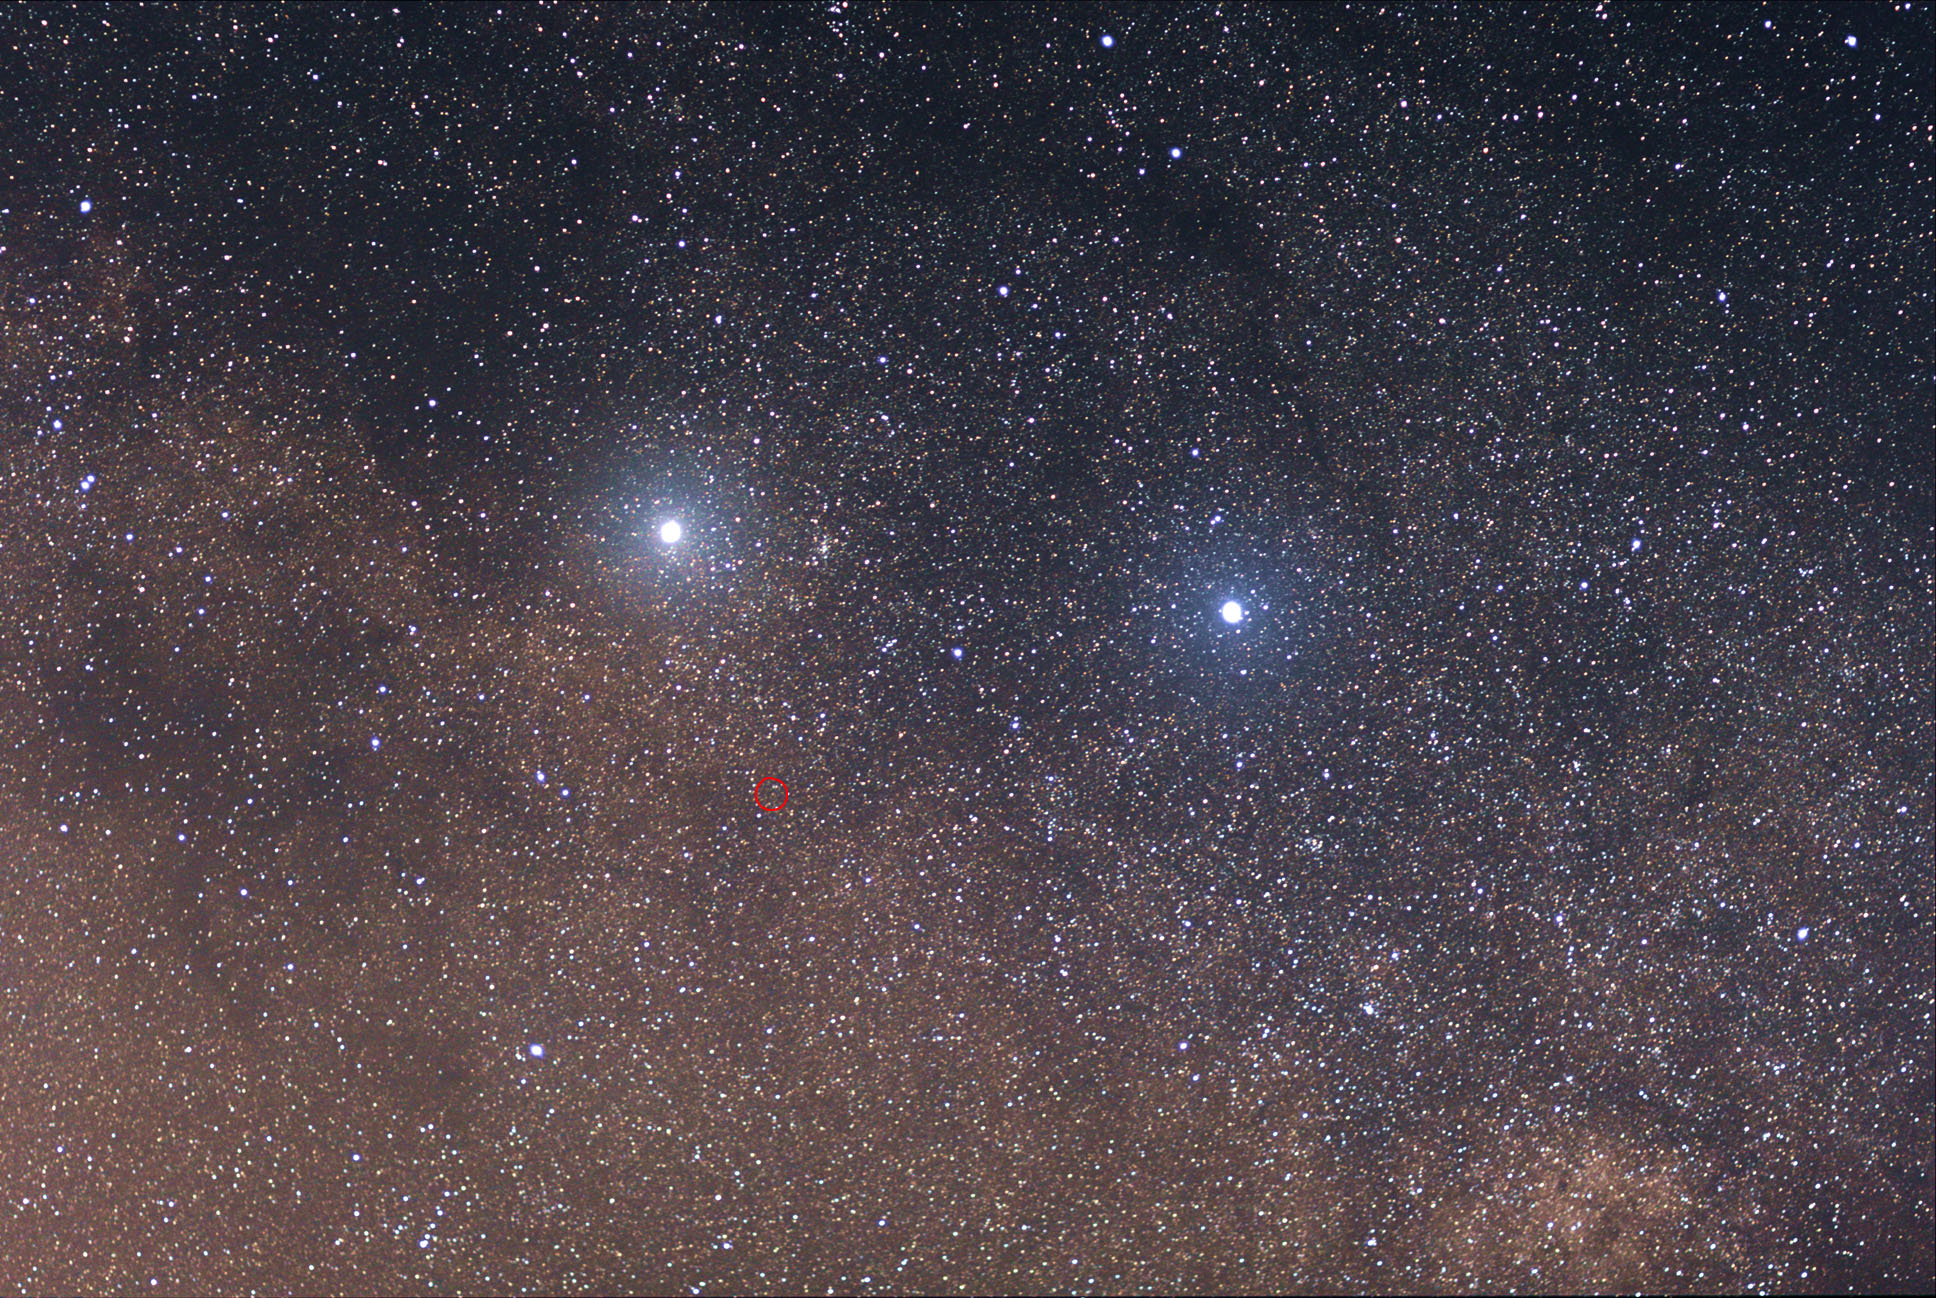
\includegraphics[width=\textwidth]{imagens/alpha-beta-proxima-centauri}
  \caption{Alpha Centauri e Beta Centauri, com Proxima circulada}
  \label{fig:estrelas}
\end{figure}
\clearpage

\section{A classe \texttt{abntex2}}
% Objetivos:
% - Apresentar a classe abntex2
% - Demonstrar como deixar este documento compatível com a ABNT

A descrição oficial do \href{http://www.abntex.net.br/}{abnTeX2} é:

\begin{quotation}
  O abnTeX2, evolução do abnTeX (ABsurd Norms for \TeX), é uma suíte para \LaTeX{} que atende os requisitos das normas da \textsc{abnt} (Associação Brasileira de Normas Técnicas) para elaboração de documentos técnicos e científicos brasileiros, como artigos científicos, relatórios técnicos, trabalhos acadêmicos como teses, dissertações, projetos de pesquisa e outros documentos do gênero.

  A suíte abnTeX2 é composta por uma classe, por pacotes de citação e de formatação de estilos bibliográficos, por exemplos, modelos de documentos e por uma ampla documentação.
\end{quotation}

Para utilizar o abnTeX2, devemos utilizar a classe \texttt{abntex2}. Ela implementa comandos e ambientes novos, como por exemplo:

\begin{multicols}{2}
  \begin{itemize}
    \item \code+\titulo+
    \item \code+\autor+
    \item \code+\orientador+
    \item \code+\instituicao+
    \item \code+\imprimircapa+
    \item \texttt{citacao} (ambiente)
    \item \texttt{resumo} (ambiente)
  \end{itemize}
\end{multicols}

\subsection{Exemplo: adaptando este documento}

Vamos adaptar este documento para a classe \texttt{abntex2}. Para isso, precisaremos:

\begin{itemize}
  \item Mudar a classe de \texttt{article} para \texttt{abntex2} e adicionar a opção \texttt{article}
  \item Alterar os comandos de metadado usando os comandos apropriados em português
  \item Substituir \verb+\maketitle+ por \verb+\imprimircapa+ ou algo parecido.
\end{itemize}

\section{Bibliografias}
% Objetivos:
% - Apresentar a maneira como bibliografias são armazenadas e utilizadas no LaTeX

Bibliografias em \LaTeX{} são organizadas em um arquivo \texttt{.bib} externo ao arquivo que contém o texto. Esse arquivo \texttt{.bib} será alimentado (manual ou automaticamente) com entradas bibliográficas, como por exemplo:

\begin{example}
  \begin{minted}[autogobble]{bibtex}
    @book{chomsky1995,
      title={The Minimalist Program},
      author={Chomsky, N.},
      series={Current studies in linguistics series},
      publisher={MIT Press},
      address={Cambridge},
      year=1995
    }
  \end{minted}
\end{example}

No arquivo principal, no local em que desejamos incluir a bibliografia, usamos o comando \code+\bibliography{arquivo}+. No decorrer do texto, podemos utilizar os comandos \code+\cite[p.~20]{greenwade93}+ e \code+\citeonline+, por exemplo, para fazer referência à entrada bibliográfica desejada. Um arquivo \texttt{bst} fica responsável pelo estilo correto da citação e da bibliografia. O pacote \texttt{abntex2cite} implementa um estilo \texttt{bst} que segue as determinações da \textsc{abnt}.

\subsection{Exemplo: bibliografia e citação}

Para incluir uma bibliografia a este arquivo, basta descomentar o pacote \texttt{abntex2cite} no preâmbulo, o comando \code+\bibliography+ e o parágrafo a seguir.

% Segundo \citeonline{chomsky1995}, …
% \bibliography{bibliografia}

\section{Macros}
% Objetivos:
% - Entender macros de substituição e macros com argumentos
% - Aprender a declarar novos ambientes

Uma das maiores vantagens do \LaTeX{} em relação aos outros editores de texto é a sua extensibilidade. É possível adicionar funcionalidades ao sistema por meio de macros. O próprio \LaTeX{} não passa de um conjunto (bastante complexo) de macros do \TeX.

Essas macros são programas que automatizam certas funções e permitem que o autor foque em escrever, ao invés de realizar tarefas tediosas repetidamente.

\subsection{Macros de substituição}

O tipo mais simples de macro é o de substituição:

\begin{example}
\mint{latex}{\newcommand{\forma}{\textsf{ForMA}}}
\end{example}

Declarações do tipo \code+\newcommand+ costumam ficar no preâmbulo do documento, para estarem disponíveis por todo o código. Após declarar o comando anterior, podemos usar \code+\forma+ com a garantia de que o texto nunca terá erros de digitação.

Ao utilizar esta macro, é necessário incluir um espaço antes do resto do texto, ou o espaço em branco será engolido: \code+\forma{} texto+. Isso ocorre, pois o \LaTeX{} está esperando um argumento. No entanto, é possível carregar o pacote \texttt{xspace}, que adiciona esse espaço de maneira automática:

\begin{example}
  \begin{minted}[autogobble]{latex}
    \usepackage{xspace}
    \newcommand{\forma}{\textsf{ForMA}\xspace}
  \end{minted}
\end{example}

\subsection{Macros com argumentos}

Já encontramos muitos comandos que levam argumentos, como por exemplo \code+\textbf{}+. Digamos, por exemplo, que nosso texto é repleto de palavras em inglês, que desejamos diferenciar do resto do texto usando itálico (ou romanas, quando o texto ao redor for itálico) e, além disso, garantir que serão hifenizadas de acordo com as regras da língua inglesa, quando ocorrerem ao fim de uma linha. Podemos declarar um comando \code+\eng{}+ facilmente, da seguinte maneira:

\begin{example}
  \begin{minted}[autogobble]{latex}
    \newcommand{\eng}[1]{%
      \emph{\foreignlanguage{english}{#1}}%
    }
  \end{minted}
\end{example}

Onde \texttt{1} indica a quantidade de argumentos que nosso comando irá receber e \texttt{\#1} será substituído pelo argumento provido pelo usuário:

\begin{example}
  \begin{minted}[autogobble]{latex}
    Por exemplo, este texto contém \eng{some words in English
    that might be hypenated correctly} caso o texto quebre
    naquela parte.
  \end{minted}
  \tcblower
  Por exemplo, este texto contém \eng{some words in English that might be hypenated correctly} caso o texto quebre naquela parte.
\end{example}

\subsection{Novos ambientes}

Também é possível definir um ambiente novo:

\begin{example}
\mint{latex}{\newenvironment{nome}[num]{antes}{depois}}
\end{example}

Por exemplo:

\begin{example}
  \begin{minted}[autogobble]{latex}
    \newenvironment{spotlight}
    {
      \vspace{1em}
      \noindent\rule{\linewidth}{.5pt}\par\vspace{5pt}
      \noindent\ignorespaces
    }
    {
      \par
      \noindent\rule{\linewidth}{.5pt}
      \vspace{1em}\ignorespacesafterend
    }
  \end{minted}
\end{example}

% Declaração do novo ambiente spotlight
\newenvironment{spotlight}
{
  \vspace{1em}
  \noindent\rule{\linewidth}{.5pt}\par\vspace{5pt}
  \noindent\ignorespaces
}
{
  \par
  \noindent\rule{\linewidth}{.5pt}
  \vspace{1em}\ignorespacesafterend
}

Veja o resultado do ambiente \texttt{spotlight}:

\begin{spotlight}
  O cuidado em identificar pontos críticos no entendimento das metas propostas
  pode nos levar a considerar a reestruturação dos conhecimentos estratégicos
  para atingir a excelência. Todavia, a valorização de fatores subjetivos
  talvez venha a ressaltar a relatividade das formas de ação.
\end{spotlight}

\subsection{Exercício: automatizando com macros}
% Problema: o texto a seguir precisa de várias macros que ainda não foram definidas. Vamos criá-las, de acordo com as seguintes especificações:
%
% - A macro \address deve conter o endereço do IEL: R. Sérgio Buarque de Holanda, 571 - Cidade Universitária, Campinas - SP
% - A macro \telephone deve expandir para (19) 3521-1502.
% - A macro \email{} deve aceitar um email como argumento e transformá-lo num link clicável. Além disso, ele deve ser formatado usando \texttt.
% - A macro \todo{} deve aceitar um argumento e mudar a cor de fundo para amarelo (“yellow”) para chamar a atenção do leitor do documento. Ele deve usar o comando \colorbox{cor}{texto} provido pelo pacote xcolor.

% Defina abaixo o comando \address

% Defina abaixo o comando \telephone

% Defina abaixo o comando \email{}

% Defina abaixo o comando \todo{}

(Crie os comandos necessários e então descomente o texto abaixo.)

% Estamos aprendendo \LaTeX{} no \ForMA. A seguir, vamos testar algumas substituições de texto e macros. Veja, por exemplo, como entrar em contato por carta, telefone ou email:

% \begin{itemize}
%   \item Endereço: \address
%   \item Telefone: \telephone
%   \item Email: \email{forma@iel.unicamp.br}
% \end{itemize}

% Este exercício ainda não está completo. Não se esqueça \todo{de criar todas as macros} e \todo{modificar o título de acordo com as especificações}.

\section{Linguística}
% Objetivos:
% - Inserir transcrições fonéticas com e sem o pacote tipa
% - Criar árvores sintáticas usando o pacote forest
% - Inserir exemplos e glosas

Os linguistas usuários de \LaTeX{} já escreveram uma série de pacotes que ajudam em tarefas de tipografia comuns à nossa área. Veremos abaixo como escrever transcrições fonéticas com o \textsc{ipa} de maneira fácil; como inserir árvores sintáticas que não são imagens e por isso não perdem resolução ao serem impressas; e como inserir exemplos, glosas e fazer referências a esses elementos no texto.

\subsection{Transcrições fonéticas}

O \href{https://ctan.org/pkg/tipa}{pacote \texttt{tipa}} permite transcrever usando o Alfabeto Fonético Internacional (\textsc{ipa}) sem ter que procurar e inserir símbolos a partir de uma lista. Tudo o que for escrito dentro do comando \code+\textipa{}+ será convertido automaticamente, seguindo uma tabela de referência intuitiva (veja o documento \texttt{tipachart.pdf}). Por exemplo, para produzir \textipa{l\~\i N.\textprimstress g\super wis.t5s}, basta digitar:

\begin{example}
  \begin{minted}[autogobble]{latex}
    \textipa{l\~\i N.\textprimstress g\super wis.t5s}
  \end{minted}
\end{example}

Alguns exemplos de vogais orais e nasais:

\begin{example}
  \begin{tabular}[h]{lr}
  \textipa{[i e E a O o u]} & \textipa{[I U 5]} \\
  \textipa{[\~o \~\textschwa{} \~5]} &
  \end{tabular}

\end{example}

E também algumas consoantes:

\begin{example}
  \begin{multicols}{2}
    \textipa{S}\\
    \textipa{Z}\\
    \textipa{L}\\
    \textipa{\textltailn}\\
    \textipa{N}\\
    \textipa{\textfishhookr}\\
    \textipa{\textturnr}\\
    \textipa{\t{tS}}\\
    \textipa{\t{dZ}}
  \end{multicols}
\end{example}

Ainda é possível inserir diagramas de vogais de maneira bastante simples,
usando o pacote \texttt{vowel}. O diagrama a seguir é idêntico ao que pode ser
encontrado na última versão do \textsc{ipa}:

\begin{center}
  \begin{vowel}
    \large
    \putcvowel[l]{i}{1}
    \putcvowel[r]{y}{1}
    \putcvowel[l]{e}{2}
    \putcvowel[r]{\o}{2}
    \putcvowel[l]{\textepsilon}{3}
    \putcvowel[r]{\oe}{3}
    \putcvowel[l]{a}{4}
    \putcvowel[r]{\textscoelig}{4}
    \putcvowel[l]{\textscripta}{5}
    \putcvowel[r]{\textturnscripta}{5}
    \putcvowel[l]{\textturnv}{6}
    \putcvowel[r]{\textopeno}{6}
    \putcvowel[l]{\textramshorns}{7}
    \putcvowel[r]{o}{7}
    \putcvowel[l]{\textturnm}{8}
    \putcvowel[r]{u}{8}
    \putcvowel[l]{\textbari}{9}
    \putcvowel[r]{\textbaru}{9}
    \putcvowel[l]{\textreve}{10}
    \putcvowel[r]{\textbaro}{10}
    \putcvowel{\textschwa}{11}
    \putcvowel[l]{\textrevepsilon}{12}
    \putcvowel[r]{\textcloserevepsilon}{12}
    \putcvowel{\textsci\ \textscy}{13}
    \putcvowel{\textupsilon}{14}
    \putcvowel{\textturna}{15}
    \putcvowel{\ae}{16}
  \end{vowel}
\end{center}

\subsection{Digitar transcrições diretamente}

Uma alternativa é utilizar a fonte \href{https://en.wikipedia.org/wiki/Doulos_SIL}{Doulos SIL}, que foi especialmente concebida para representar corretamente todos os glifos usados na transcrição. Basta configurá-la no preâmbulo como a fonte para entrada de texto em \textsc{ipa} e digitar a transcrição diretamente no código-fonte:

\begin{example}
  \begin{minted}[autogobble]{latex}
    % No preâmbulo do documento:
    \newfontfamily\ipafont{Doulos SIL}
    % …e no corpo do documento (veja o código-fonte, pois esta
    % fonte não é capaz de exibir todos os caracteres):
    {\ipafont [ʃøɔũʸᵃᵐᶺɹɾɽʏɭɮʄʑʐʝʃħɦʒ]}
  \end{minted}
  \tcblower
  Resultado: {\ipafont [ʃøɔũʸᵃᵐᶺɹɾɽʏɭɮʄʑʐʝʃħɦʒ]}
\end{example}

\subsection{Árvores sintáticas com o \texttt{forest}}

Existem muitos pacotes para a inserção de árvores sintáticas no \LaTeX, mas provavelmente o melhor e mais poderoso é o \href{https://ctan.org/pkg/forest}{\texttt{forest}}. Para inserir uma árvore, basta iniciar o ambiente forest e inserir uma sentença com os constituintes delimitados por chaves. Ela será convertida automaticamente para uma árvore.

\begin{example}
  \begin{minted}[autogobble]{latex}
    \begin{forest}
      [CP [C] [IP [I] [VP [V] [NP] ] ] ]
    \end{forest}
  \end{minted}
  \tcblower
  \begin{forest}
    [CP [C] [IP [I] [VP [V] [NP] ] ] ]
  \end{forest}
\end{example}

Por motivos de legibilidade do código, devemos pular linhas e indentar os constituintes que estão em níveis mais baixos da árvore (␣ representa um espaço em branco):

\begin{example}
  \begin{minted}[autogobble]{latex}
    \begin{forest}
      ␣␣[CP
      ␣␣␣␣[C]
      ␣␣␣␣␣␣[IP
      ␣␣␣␣␣␣␣␣[I]
      ␣␣␣␣␣␣␣␣[VP
      ␣␣␣␣␣␣␣␣␣␣[V]
      ␣␣␣␣␣␣␣␣␣␣[NP]
      ␣␣␣␣␣␣␣␣]
      ␣␣␣␣␣␣]
      ␣␣]
    \end{forest}
  \end{minted}
\end{example}

A árvore a seguir (veja o código-fonte) é um exemplo com todos os nós rotulados e com os nós terminais precedidos de linhas. Note como os nós terminais estão marcados como constituintes dentro de outros constituintes, por exemplo em \code+[DP [O menino]]+. Note, ainda, que \code+$_i$+ significa que estamos entrando no modo de matemática (\code+$…$+) e inserindo um \emph{i} subscrito (\code+_i+):

\begin{example}
  \begin{forest}
  [IP
    [DP [O menino$_i$]]
    [I$'$
      [I [chegou$_j$]]
      [VP
      [V$'$
        [V [t$_j$]]
        [DP [t$_i$]]
      ]
      ]
    ]
  ]
\end{forest}
\end{example}

É bastante usual omitirmos as linhas que levam aos nós terminais, pois algumas pessoas as consideram redundantes. Isso é possível usando uma sintaxe ligeiramente diferente. Note que, agora, há uma quebra de linha e apenas um constituinte em \code+[DP\\ O menino]+, por exemplo:

\begin{example}
\begin{forest}
  [IP
    [DP\\ O menino$_i$]
    [I$'$
      [I\\ chegou$_j$]
      [VP
        [V$'$
          [V\\ t$_j$]
          [DP\\ t$_i$]
        ]
      ]
    ]
  ]
\end{forest}
\end{example}

O pacote \texttt{forest} é baseado no \href{https://en.wikipedia.org/wiki/PGF/TikZ}{PGF/TikZ}, um conjunto de bibliotecas gráficas para o \LaTeX. Como consequência, as árvores aceitam uma série de customizações que não discutiremos no momento. Porém, vejamos um exemplo para ilustrar o que se pode esperar encontrar no manual do \texttt{forest}. A árvore a seguir não tem todos os nós rotulados e isso causa um comportamento estranho quando a árvore é disposta na página. No entanto, podemos usar a opção for \texttt{tree = nice empty nodes} para remediar a situação:

\begin{example}
\begin{forest}
  for tree=nice empty nodes
  [
    [
      [a]
      [menina]
    ]
    [
      [comeu]
        [
          [o]
          [bolo]
        ]
    ]
  ]
\end{forest}
\end{example}

Essa opção, porque se encontra dentro do ambiente \texttt{forest}, irá se aplicar somente para a árvore em questão. Veja o manual do pacote para mais opções.

Às vezes, desejamos omitir informações irrelevantes em alguma árvore. Explicitamos nossa decisão desenhando um triângulo sobre o constituinte que não foi esmiuçado. Para isso, usamos a opção \texttt{roof}, que se aplica a um constituinte em nossa árvore. Veja no exemplo a seguir, onde o constituinte [chutada pelo menino] está simplificado:

\begin{example}
\begin{forest}
  [IP
    [DP\\ a bola]
    [I$'$
      [I\\ foi]
      [VP
        [V$'$
          [V]
          [PartP [chutada pelo\\ menino, roof]]
        ]
      ]
    ]
  ]
\end{forest}
\end{example}

\subsection{Exemplos numerados e glosas com o \texttt{linguex}}

Outra tarefa especialmente comum para o linguista é apresentar seus dados em formato de exemplos de sentenças, que são numeradas à esquerda. Não existe uma implementação perfeita em \LaTeX{} para isso, pois cada uma tem suas vantagens e defeitos. O \href{https://ctan.org/pkg/linguex}{\texttt{linguex}} é um desses pacotes com suporte a exemplos e glosas. Você pode aprender sobre outros pacotes para linguistas \href{https://en.wikibooks.org/wiki/LaTeX/Linguistics}{nesse artigo da WikiBooks}, caso o \texttt{linguex} não tenha as funcionalidades de que precisa.

Escolhemos o \texttt{linguex} pois sua sintaxe é relativamente simples e poderosa. Vejamos alguns exemplos básicos:

% não consegui colocar no ambiente example
\ex. Chegou o menino.

\ex. Chegou a carta.

\ex.* A chegou carta.

Sempre deixe uma linha em branco para indicar o fim de um exemplo. É possível mostrar também subexemplos:

% não consegui colocar no ambiente example
\ex.
  \a. Chegou o menino.
  \b. O menino chegou.

Novamente, certifique-se de colocar uma linha em branco ao final dos exemplos.

Também é possível escrever glosas usando o comando \code+\exg.+. As palavras serão alinhadas automaticamente:

\exg.
  Gila abur-u-n ferma hamišaluǧ güǧüna amuq’-da-č.\\
  now they-OBL-GEN farm forever behind stay-FUT-NEG\\
  ``Now their farm will not stay behind forever.''

\subsubsection{Referências cruzadas}

Já vimos que os comandos \code+\label+ e \code+\ref+ permitem criar referências que são automaticamente numeradas e atualizadas pelo \LaTeX. Esses comandos também funcionam nos exemplos e glosas do \texttt{linguex}:

\ex.\label{ex:gram} Chegou o menino.

\ex.*\label{ex:agram} A chegou carta.

Em~\ref{ex:gram}, temos uma sentença bem formada, ao contrário de~\ref{ex:agram}, que é uma sentença agramatical.

% Obrigado por participar!
\vfill
\begin{center}
  \begin{tcolorbox}[width=.4\textwidth,
    colback=yellow!5!white,
    colframe=yellow!75!white,
    halign=center,
    valign=center,
    square,
    circular arc]
    \Large\sffamily Isso é tudo,\\ pessoal! \emoji{winking-face-with-tongue}
  \end{tcolorbox}
\end{center}
\end{document}
